
\labsection{Линейные фильтры. Гармонические колебания. Частотная характеристика}

\todo [author=Tiffani]{Нет подписи ко всем рисункам в главе, только номер}
\todo [author=Tiffani]{На всех рисунках некорректные обозначения. psfrag не работает}


Во многих случаях реальные электрические системы (например, колебательный контур, показанный на рис.~\figref{RLC circuit}) ведут себя как линейные фильтры.

\begin{wrapfigure}{r}{0.35\textwidth}
	\psfrag{f}[cc]{$f(t)$}
	\psfrag{g}[cl]{$g(t)$}
	\psfrag{r}[ct]{$R$}
	\psfrag{c}[cr]{$C$}
	\psfrag{l}[cb]{$L$}
	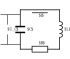
\includegraphics[width=0.3\textwidth]{Chapter_6/1}
	\caption{}
	\figmark{RLC circuit}
\end{wrapfigure}

Напомним, фильтр называется линейным, если имеет место принцип суперпозиции: отклик фильтра на сумму внешних воздействий
равен сумме откликов на каждое воздействие.

Например, закон Кирхгофа для последовательного колебательного контура (сумма падений напряжений на всех участках
замкнутого контура равна сумме ЭДС) имеет вид

\begin{equation*}
	L\ddot{q}+\dot{q}R+\frac{q}{C}=f(t),
\end{equation*}
где $q(t)$~--- заряд конденсатора, $f(t)$~--- внешняя ЭДС, возбуждающая колебания в контуре. Для выходного сигнала
(напряжение на конденсаторе $g(t)=q/C$) получаем уравнение

\begin{equation*}
	\ddot{g}+2\delta\dot{g}+\omega_0^2 g=\omega_0^2 f(t),
\end{equation*}
где $\delta=R/2L$, $\omega_0^2=1/LC$.

Пусть $g_1(t)$~--- выходной сигнал контура при входном сигнале (внешней ЭДС) $f_1(t)$, тогда

\begin{equation*}
	\ddot{g}_1+2\delta \dot{g}_1 +\omega_0^2 g_1=\omega_0^2 f_1(t).
\end{equation*}

При внешней ЭДС $f_2(t)$ выходной сигнал есть $g_2(t)$

\begin{equation*}
	\ddot{g}_2+2\delta \dot{g}_2+\omega_0^2g_2=\omega_0^2 f_2(t).
\end{equation*}

Пусть теперь внешняя ЭДС является линейной суперпозицией воздействий $f_1(t)$ и $f_2(t)$, т.~е.

\begin{equation*}
	f(t)=c_1f_1(t)+c_2f_2(t),
\end{equation*}
тогда выходной сигнал фильтра $g(t)$ подчиняется уравнению

\begin{equation*}
	\ddot{g}+2\delta\dot{g}+\omega_0^2g=\omega_0^2[c_1f_1(t)+c_2f_2(t)].
\end{equation*}

Домножив левые и правые части уравнений для $g_1(t)$ и $g_2(t)$ на $c_1$ и $c_2$ соответственно и сложив их, получим,
что сигнал $g(t)$ может быть представлен в виде

\begin{equation*}
	g(t)=c_1g_1(t)+c_2g_2(t),
\end{equation*}
т.~е. принцип суперпозиции справедлив.

Обобщая сказанное, изобразим произвольную линейную систему (фильтр) с помощью блок-схемы:

\begin{equation*}
	f(t)\to\fbox{$L$} \to g(t),
\end{equation*}
где $f(t)$~--- внешнее воздействие (входной сигнал фильтра), например, внешняя ЭДС, действующая на колебательный контур,
$g(t)$~--- выходной сигнал (отклик фильтра), например, напряжение на конденсаторе контура.

Равенство $g(t)=L[f(t)]$ означает, что выходной сигнал $g(t)$ есть результат действия линейной системы на входной сигнал $f(t)$. 

%Правки. Локшин
%Тогда свойство линейности (принцип суперпозиции) можно символически записать в виде равенства
%\begin{equation*}
%L[c_1f_1(t)+c_2f_2(t)]=c_1L[f_1(t)]+c_2L[f_2(t)].
%\end{equation*}

Мы будем рассматривать далее \important{линейные стационарные фильтры,} т.~е. линейные фильтры с постоянными, не зависящими от
времени параметрами $L$, $C$, $R$. Такие фильтры описываются линейными уравнениями с \important{постоянными} коэффициентами.

Из свойства линейности следует простое правило для нахождения отклика фильтра на произвольное внешнее воздействие $f(t)$:
необходимо представить это воздействие в виде суперпозиции некоторых элементарных слагаемых, а затем найти отклик на
каждое слагаемое. Окончательный результат получается суммированием откликов. В этом состоит суть спектрального подхода к
решению задачи линейной фильтрации.

Выбор базиса (элементарных слагаемых) неоднозначен. Естественно попытаться разложить внешнее воздействие на такие
слагаемые, отклик на которые находится наиболее простым образом. Такими слагаемыми являются так называемые
\important{собственные функции фильтра}, т.~е. функции $\Psi_n(t)$, удовлетворяющие равенству

\begin{equation*}
	L[\Psi_n(t)]=H_n\Psi_n(t).
\end{equation*}

Это равенство означает, что, если внешнее воздействие описывается собственной функцией, то отклик описывается той же
функцией (с некоторым множителем $H_n$, который математики называют собственным значением).

Для линейных стационарных фильтров такими собственными функциями являются функции $e^{i\omega t}$~--- гармонические
колебания, записанные в комплексной форме:

\begin{equation*}
	L\left[e^{i\omega t}\right]=H(\omega)e^{i\omega t},
\end{equation*}
причём каждой частоте $\omega$ соответствует своё собственное значение (т.~е. множитель $H$ является функцией частоты
$\omega$: $H=H(\omega)$). Эту в общем случае комплексную функцию $H(\omega)=A(\omega)e^{i\varphi(\omega)}$ называют в физике
\important{частотной характеристикой} (или \important{передаточной функцией}) фильтра.

Функцию $A(\omega)=|H(\omega)|$ называют \important{амплитудной характеристикой} фильтра (амплитуда вынужденных колебаний в
функции частоты $\omega$), а функцию $\varphi(\omega)= arg H(\omega)$ называют \important{фазовой характеристикой} (сдвиг по фазе
вынужденных колебаний относительно внешнего гармонического воздействия $e^{i\omega t}$).

%Правки. Локшин
%\important{Задача 1.} Найти частотную характеристику $H(\omega)$ фильтра, изображённого на рис. \figref{RLC circuit}. Показать, что функция $e^{i\omega t}$ является собственной функцией этого фильтра.

%Частотная характеристика определяет отклик на входной гармонический сигнал единичной амплитуды~--- внешнюю ЭДС $e^{i\omega t}$.

%\begin{wrapfigure}[24]{r}{0.35\textwidth}
	%\psfrag{x}{$\omega$}
	%\psfrag{y}{$|H(\omega)|$}
	%\psfrag{o}[tc]{0}
	%\psfrag{t}[tc]{$\omega_0$}
	%\psfrag{d}[cb]{$2\delta$}
	%\psfrag{q}[cr]{$Q$}
%	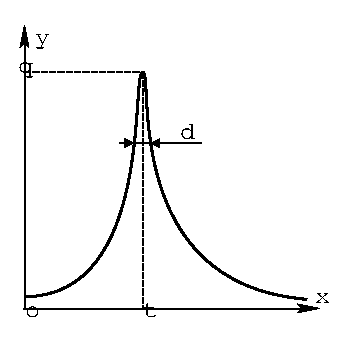
\includegraphics[width=0.25\textwidth]{R2}
%	\caption{}
%	\figmark{6.2}
%\end{wrapfigure}
%
%Закон Кирхгофа:

%\begin{equation*}
%\dot{q}R+\frac{q}{C}+L\ddot{q}=e^{i\omega t}.
%\end{equation*}
%Для выходного сигнала $g(t)=\frac{q}{C}$ получаем уравнение

%\begin{equation*}
%\ddot{g}+2\delta\dot{g}+\omega_0^2g=\omega_0^2 e^{i\omega t}.
%\end{equation*}
%Ищем решение (\r{2}) в виде

%\begin{equation*}
%g(t)=H(\omega)e^{i\omega t}.
%\end{equation*}
%Подставляя в (\r{2}), имеем (поскольку $\dot{g}(t)=i\omega H(\omega)e^{i\omega t}$,
%$\ddot{g}=(i\omega)^2H(\omega)e^{i\omega t})$:

%\begin{equation*}
%-\omega^2H(\omega)+2\delta(i\omega)H(\omega)+\omega_0^2 H(\omega)=\omega_0^2.
%\end{equation*}
%Окончательно находим:

%\begin{equation*}
%H(\omega)=\frac{\omega_0^2}{\omega_0^2-\omega^2+i2\delta\omega},
%\end{equation*}

%\begin{equation*}
%\left|H(\omega)\right|=\frac{\omega_0^2}{\sqrt{(\omega_0^2-\omega^2)^2+4\delta^2\omega^2}}~(рис. \figref{6.2}),\qquad
%\varphi(\omega)=-\arctg\frac{2\delta\omega}{\omega_0^2-\omega^2}.
%\end{equation*}


\labsection{Векторное представление гармонических колебаний}

\begin{wrapfigure}[]{r}{0.35\textwidth}
	\psfrag{x}{$x$}
	\psfrag{0}[cb]{0}
	\psfrag{a}[br]{$a$}
	\psfrag{s}{$\mathbf{S}$}
	\psfrag{f}{$\varphi_0$}
	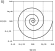
\includegraphics[width=0.25\textwidth]{Chapter_6/3}
	\caption{}
	\figmark{vec-harm-osc}
\end{wrapfigure}

Напомним, что гармоническое колебание
\begin{equation*}
	f(t)=a\cos(\omega t+\varphi_0)
\end{equation*}
изображают вектором $\vec{S}$, длина которого равна амплитуде колебания $a$, а угол между вектором и горизонтальной осью
$x$~--- начальной фазе колебания $\varphi_0$ (рис.~\figref{vec-harm-osc}). При этом частота $\omega$ гармонического колебания предполагается
заданной. Смысл этого представления состоит в следующем.

\begin{wrapfigure}[]{r}{0.35\textwidth}
	\psfrag{o}[cb]{0}
	\psfrag{f}[cc]{$\varphi_1$}
	\psfrag{F}[cc]{$\varphi_2$}
	\psfrag{a}[tl]{$\mathbf{S}_1$}
	\psfrag{b}[tl]{$\mathbf{S}_2$}
	\psfrag{c}[br]{$\mathbf{S}$}
	\psfrag{d}[br]{$a_1$}
	\psfrag{e}[br]{$a_2$}
	\psfrag{g}[br]{$a$}
	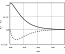
\includegraphics[width=0.25\textwidth]{Chapter_6/4}
	\caption{}
	\figmark{harm osc - sum}
\end{wrapfigure}

Вообразим, что вектор $\vec{S}$ вращается вокруг точки $O$ с угловой скоростью $\omega$ против часовой стрелки (а мы
сделали мгновенную фотографию в момент $t=0$, когда угол наклона вектора $\Phi(t)=\omega t + \varphi_0$ равен $\varphi_0$).
Заметим, что проекция вектора $\vec{S}$ на ось $x$ при вращении изменяется по закону $f(t)=a\cos(\omega t+\varphi_0)$, т.~е.
совершает гармонические колебания.

Геометрическое изображение гармонического колебания $f(t)$ в виде вектора $\vec{S}$ удобно использовать при решении задачи
сложения колебаний. Пусть мы имеем две скалярные величины $f_1$ и $f_2$, изменяющихся по гармоническому закону с
одинаковой частотой $\omega$:

\begin{equation*}
	f_1(t)=a_1\cos(\omega t+\varphi_1), \qquad f_2(t)=a_2\cos(\omega t+\varphi_2).
\end{equation*}

Необходимо найти колебание $f(t)$ (скалярную величину), являющееся суммой колебаний $f_1(t)$ и $f_2(t)$:
\begin{equation*}
	f(t)=f_1(t)+f_2(t).
\end{equation*}

Изобразим колебания $f_1(t)$ и $f_2(t)$ в виде векторов $\vec{S}_1$ и $\vec{S}_2$ (рис.~\figref{harm osc - sum}), вектор $\vec{S}$~--- суммарный вектор.
Векторы $\vec{S}_1$, $\vec{S}_2$, $\vec{S}$ образуют треугольник, причём внешний угол треугольника (угол $\Delta\varphi$ между
векторами $\vec{S}_1$ и $\vec{S}_2$) равен разности фаз колебаний $f_1$ и $f_2$. Представим себе, что векторы $\vec{S}_1$ и
$\vec{S}_2$ вращаются с одной и той же угловой скоростью $\omega$ против часовой стрелки. Ясно, что угол $\varphi$ между
векторами $\vec{S}_1$ и $\vec{S}_2$ остаётся при таком вращении неизменным, а суммарный вектор $\vec{S}$ повернётся за время
$t$ (как и $\vec{S}_1$, и $\vec{S}_2$) на угол $\omega t$, т.~е. весь треугольник векторов вращается как одно целое. Причём
очевидно, что проекция суммарного вектора $\vec{S}$ на ось $x$ в произвольный момент времени $t$ равна сумме проекций
векторов $\vec{S}_1$ и $\vec{S}_2$:

\begin{equation*}
	a\cos(\omega t + \varphi)=a_1\cos(\omega t+\varphi_1)+a_2\cos(\omega t + \varphi_2),
\end{equation*}
здесь $a$~--- длина вектора $\vec{S}$, а $\varphi$~--- его угол наклона при $t = 0$.

Итак, сумма гармонических колебаний одинаковой частоты является гармоническим колебанием той же частоты. Амплитуда $a$
суммарного колебания может быть найдена из треугольника векторов по теореме косинусов:
\begin{equation*}
	a^2=a_1^2+a_2^2+2a_1a_2\cos(\varphi_2-\varphi_1).
\end{equation*}

\labsection{Модулированные колебания. Амплитудная и фазовая модуляции}

Для передачи сигналов~--- музыки, речи, телевизионного изображения~--- необходимо нарушение синусоидальности. Отклонение
от синусоидальности и выражает содержание передаваемой информации. Колебательный процесс, отличный от гармонического,
назовём \important{модулированным колебанием}. Примеры таких процессов (их осциллограммы) приведены на рис.~\figref{modulated oscillation}.

\begin{figure}[h!]
	\psfrag{a}[ct]{а)}
	\psfrag{b}[ct]{б)}
	\psfrag{c}[ct]{в)}
	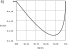
\includegraphics[width=1.0\textwidth]{Chapter_6/5}
	\caption{}
	\figmark{modulated oscillation}
\end{figure}

Будем записывать модулированные колебания в виде
\begin{equation}
	\eqmark{6.1}
	f(t)=a(t)\cos(\omega_0t+\varphi(t)).
\end{equation}

В отличие от гармонического колебания, здесь $a(t)$ и $\varphi(t)$~--- меняющиеся во времени величины. Форма записи \eqref{6.1}
особенно целесообразна в том случае, когда $a(t)$ и $\varphi(t)$~--- медленно меняющиеся функции времени, т.~е. на
интервалах времени $\tau$, существенно превышающих период гармонического (так называемого <<несущего>>) колебания
частоты $\omega_0$:
\begin{equation}
	\eqmark{6.2}
	\tau \gg \frac{2\pi}{\omega_0},
\end{equation}
эти функции остаются практически неизменными: $a(t)\approx a_{0}$ и $\varphi(t)\approx\varphi_0$. Такое колебание называется
\important{квазигармоническим}. В этом случае медленно меняющиеся величины $a(t)$ и $\varphi(t)$ принято называть амплитудой и
начальной фазой модулированного колебания.

Итак, квазигармоническое колебание можно характеризовать двумя параметрами: периодом несущего колебания
$T_0=2\pi/\omega_0$ и временем $\tau \gg T_0$, характеризующим быстроту изменения амплитуды $a(t)$ и (или) начальной
фазы $\varphi(t)$.

%Правки. Локшин
%Для передачи радиосигналов используются высокочастотные несущие колебания (от сотен килогерц до сотен мегагерц), в то время как модуляционные отклонения от синусоидальности, которые описываются функциями $a(t)$ и $\varphi(t)$, характеризуются своей медленностью, т.~е. сравнительно низкими звуковыми частотами (от десятков до тысяч герц), таким образом, неравенство \eqref{quasiharmonic oscillation - tau} выполняется, как правило, с большим запасом. 
%
Для описания модулированных колебаний используется
следующая терминология: говорят, что функция $a(t)$ описывает закон амплитудной модуляции, а функция $\varphi(t)$~--- закон
фазовой модуляции. Именно в этих функциях и заложена передаваемая информация.

Если $\varphi(t)=\varphi_0=const$, то
\begin{equation}
	\eqmark{6.3}
	f(t)=a(t)\cos(\omega_0t+\varphi_0),
\end{equation}
где $a(t)\ge0$. Такое колебание называют \important{модулированным по амплитуде.}

Если $a(t)=a_0=const$, то

\begin{equation}
	\eqmark{6.4}
	f(t)=a_0 \cos(\omega_0t+\varphi(t)).
\end{equation}

Такое колебание называют \important{модулированным по фазе.}

В общем случае имеем как амплитудную, так и фазовую модуляцию, т.~е. колебание вида \eqref{6.1}.

%Правки. Локшин
%Поставим в соответствие реальному модулированному колебанию \eqref{modulated oscillation} комплексную функцию

%\begin{equation*}
%	z(t)=a(t)e^{i[\omega_0t+\varphi(t)]}.
%\end{equation*}

%\begin{wrapfigure}[]{r}{0.35\textwidth}
	%\psfrag{a}[cb]{$e^{i\omega_0t}$}
	%\psfrag{c}{$f_0(t)e^{i\omega_0t}$}
	%\psfrag{b}{$f_0(t)$}
%	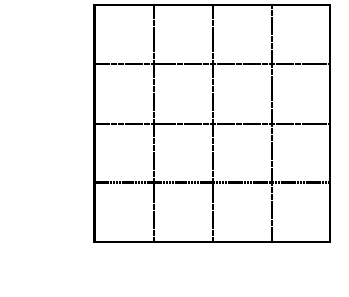
\includegraphics[width=0.25\textwidth]{2}
%	\caption{}
%	\figmark{2}
%\end{wrapfigure}

%Колебание \eqref{modulated oscillation} является действительной частью комплексной функции $z(t)$: $f(t)=\Re z(t)$. Функция $z(t)$ представляется в виде произведения функции $f_0(t)=a(t)e^{i\varphi(t)}$, содержащей всю информацию о законах модуляции $a(t)$ и $\varphi(t)$, и функции $e^{i\omega_0t}$~--- гармонического несущего колебания (записанного в комплексной форме)

%\begin{equation*}
%	z(t)=f_0(t)e^{i\omega_0t}.
%\end{equation*}
%Операцию модуляции~--- перемножение \important{модулирующего} сигнала $f_0(t)$ на \important{модулируемое} высокочастотное гармоническое колебание $e^{i\omega_0t}$~--- принято изображать в виде блок-схемы (рис. \figref{2}).

%Таким образом, непременными составными частями любой передающей радиостанции являются: генератор высокочастотного гармонического колебания $e^{i\omega_0t}$, источник сигнала $f_0(t)$, содержащего передаваемую информацию, и \important{модулятор}~--- устройство, осуществляющее их перемножение.

%\begin{wrapfigure}[]{r}{0.35\textwidth}
	%\psfrag{A}[cb]{а)}
	%\psfrag{B}[cb]{б)}
	%\psfrag{a}[cb]{$a(t)$}
	%\psfrag{b}[cb]{$a_0$}
	%\psfrag{c}[cc]{$\varphi_0$}
	%\psfrag{d}{$\varphi(t)$}
%	\includegraphics[width=0.25\textwidth]{6}
%	\caption{}
%	\figmark{6}
%\end{wrapfigure}

%Так же, как и гармонические колебания, квазигармонические процессы изображают в виде векторов. Если гармоническое колебание

%\begin{equation}
%	\eqmark{harm osc}
%	f(t)=a_0\cos(\omega_0 t+\varphi_0)
%\end{equation}
%изображается вектором $\mathbf{S}_0$, имеющим фиксированную длину $a_0$ и направление $\varphi_0$, то модулированное колебание на той же векторной диаграмме естественно изобразить в виде вектора, длина которого $a(t)$ и (или) угол наклона~--- $\varphi(t)$ медленно изменяются (медленно~--- если речь идёт о квазигармоническом колебании). В частности, амплитудно-модулированное колебание \eqref{amplitude-modulated} изображается вектором неизменного направления $\varphi_0$, длина которого изменяется (рис. \figref{6}а), а колебание \eqref{phase-modulated}, модулированное по фазе,~--- вектором неизменной длины, угол наклона которого $\varphi(t)$ изменяется (качания вектора на рис. \figref{6}б).

%Аргумент косинуса в \eqref{phase-modulated} называют \important{фазой модулированного колебания} $\varphi(t)=\omega_0t+\varphi(t)$, причём в отличие от гармонического колебания скорость изменения фазы $\dot{\Phi}$ (величина, которую можно назвать частотой $\omega$) является функцией времени

%\begin{equation}
%	\eqmark{phase-change}
%	\omega(t)=\dot{\Phi}(t)=\omega_0+\dot{\varphi}(t).
%\end{equation}

%Если выполнено условие квазигармоничности \eqref{quasiharmonic oscillation - tau}, то $\dot{\varphi}(t)\ll \omega_{0}$, т.~е. меняющаяся во времени частота $\omega (t)$ мало отклоняется от частоты $\omega_0$ гармонического колебания \eqref{harm osc}.

%Отметим также, что если $\varphi(t)$ меняется по линейному закону $\varphi(t)= \Omega t$, то мы получаем из \eqref{phase-change}

%\begin{equation}
%	\eqmark{frequency shift}
%	\omega=\omega_0+\Omega,
%\end{equation}
%т.~е. \emph{гармоническое} колебание со смещённой частотой, причём $\Omega\ll\omega_0$ при условии \eqref{quasiharmonic oscillation - tau}.

%В системе координат, в которой гармоническое колебание частоты $\omega_0$ изображается неподвижным вектором, колебание с частотой $\omega=\omega_0+\Omega$ изображается вектором, медленно вращающимся против часовой стрелки с частотой $\Omega$, если $\Omega>0$ и по часовой стрелке при $\Omega<0$.
%

Осциллограммы процессов на рис. \figref{modulated oscillation}а, б являются примерами амплитудно-модулированных колебаний, а на рис. \figref{modulated oscillation}в~--- пример
колебания, модулированного по фазе.

\labsection{Спектральное разложение}

\labsection{Действительная и комплексная форма спектральных разложений}

Итак, при изучении линейных систем (фильтров) возникает необходимость представления произвольного сигнала
(модулированного колебания) $f(t)$ в виде
\begin{equation}
	\eqmark{6.5}
	f(t)=\sum c_n e^{i\omega_n t}.
\end{equation}
Представление \eqref{6.5} называется разложением сигнала $f(t)$ в ряд Фурье, а отдельные слагаемые ряда (составляющие
гармонические колебания) $c_n e^{i\omega_n t}$ называют \important{гармониками}. Совокупность коэффициентов $c_n$ называется
спектром функции $f(t)$, при этом $|c_n|$ определяет амплитуду гармоники частоты $\omega_n$, а $arg c_n$~--- начальную
фазу.

Равенство \eqref{6.5} утверждает, что можно подобрать амплитуды и фазы слагаемых гармонических колебаний, а также их частоты
так, чтобы получить в сумме заданный сигнал $f(t)$. В дальнейшем мы будем говорить (если не делается специальных
оговорок) о сигналах, описываемых \important{действительными функциями} $f(t)$. Подробнее условия, налагаемые на функции
$f(t)$, при выполнении которых возможно разложение \eqref{6.5}, изучаются в курсах математики. Здесь же отметим
замечательные математические свойства гармонических функций.

Во-первых, гармоническое колебание $e^{i\omega_0 t}$ частоты $\omega_0$ не может быть представлено суперпозицией
гармонических колебаний $\sum c_n e^{i\omega_n t}$ других частот $\omega_n\ne\omega_0$, какие бы коэффициенты $c_n$,
т.~е. амплитуды и фазы слагаемых гармоник, мы ни старались подобрать. Математически это свойство называют
ортогональностью: функция $e^{i\omega_0 t}$ не имеет <<проекции>> на любую другую функцию $e^{i\omega_nt}$ при
$\omega_0\ne\omega_n$, подобно тому как вектор, параллельный оси $z$, невозможно представить в виде суммы векторов,
параллельных осям $x$ и $y$.

Второе важнейшее математическое свойство~--- единственность представления \eqref{6.5}: существует единственный набор
необходимых частот $\omega_n$ и единственный набор отвечающих этим частотам амплитуд $a_n$ и фаз $\varphi_n$, обеспечивающих
представление функции $f(t)$ в виде суперпозиции гармонических функций. Наконец, не вдаваясь в математические детали,
отметим ещё одно важное обстоятельство: любой физически реализуемый колебательный процесс может быть представлен в виде
суммы (быть может, в виде непрерывной суммы~--- интеграла) гармонических колебаний.

Наряду с разложением \eqref{6.5} часто используется разложение действительных функций в ряд Фурье вида

\begin{equation}
	\eqmark{6.6}
	f(t)=\sum a_n \cos(\omega_n t+\varphi_n ).
\end{equation}

Какова связь между коэффициентами этих разложений: комплексным коэффициентом $c_n$ и действительными числами $a_n$,
$\varphi_n$? Каждое слагаемое ряда \eqref{6.6} можно с помощью формулы Эйлера:

\begin{equation*}
	\cos\alpha=\frac{e^{i\alpha}+e^{-i\alpha}}{2}
\end{equation*}
представить в виде

\begin{equation*}
	a_n\cos(\omega_nt+\varphi_n)=\frac{a_n}{2}e^{i\varphi_n}\,e^{i\omega_n t}+\frac{a_n}{2}e^{-i\varphi_n}\,e^{-i\omega_n t},
\end{equation*}
откуда ясно, что разложения \eqref{6.5} и \eqref{6.6} будут тождественны, если суммирование в \eqref{6.5} проводить как по
положительным частотам $\omega_n$ (имеющим понятный физический смысл), так и по отрицательным (формально введённым)
частотам~--- $\omega_n$, причём соответствующие коэффициенты имеют вид

\begin{equation}
	\eqmark{6.7}
	c_n =\frac{1}{2}a_n e^{i\varphi_n}, \qquad c_{-n}=\frac{1}{2}a_n e^{-i\varphi_n}
\end{equation}
(коэффициенты $c_{-n}$ соответствуют отрицательным частотам $-\omega_n)$, т.е каждому слагаемому $a_n\cos(\omega_nt+\varphi_n)$
ряда \eqref{6.6} соответствуют два слагаемых $c_ne^{i\omega_n t}$ и $c_{-n}e^{-i\omega_n t}$ ряда \eqref{6.5}.

\begin{wrapfigure}{r}{0.35\textwidth}
	\psfrag{a}[ct]{$\omega_1$}
	\psfrag{b}[ct]{$\omega_2$}
	\psfrag{c}[ct]{$\omega_3$}
	\psfrag{d}[ct]{$\omega_4$}
	\psfrag{e}[ct]{$-\omega_{1}$}
	\psfrag{f}[ct]{$-\omega_{2}$}
	\psfrag{g}[ct]{$-\omega_{3}$}
	\psfrag{h}[ct]{$-\omega_{4}$}
	\psfrag{o}[ct]{0}
	\psfrag{1}[cb]{$\varphi_1$}
	\psfrag{2}[cb]{$\varphi_2$}
	\psfrag{3}[cb]{$\varphi_3$}
	\psfrag{4}[cb]{$\varphi_4$}
	\psfrag{x}{$\w$}
	\psfrag{y}{$\{c_n\}$}
	\psfrag{z}{$\{a_n\}$}
	\psfrag{A}{а)}
	\psfrag{B}{б)}
	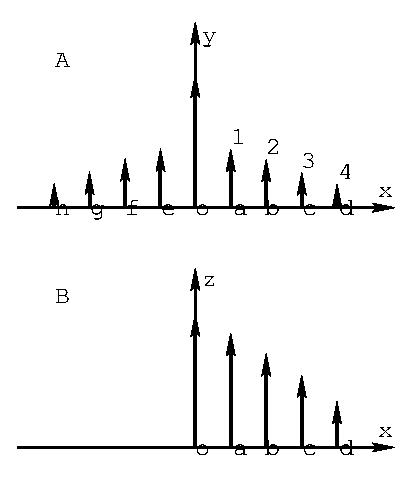
\includegraphics[width=0.25\textwidth]{Chapter_6/7}
	\caption{}
	\figmark{spectrum}
\end{wrapfigure}

Мы видим, что при разложении действительных функций $f(t)$ в ряд Фурье коэффициенты разложения $c_{-n}$ на отрицательных
частотах связаны с коэффициентами $c_n$ простым соотношением $c_n=c_{-n}^*$, т.~е. являются комплексно-сопряжёнными.
Таким образом, гармоники с отрицательными частотами не несут какой-либо дополнительной информации о сигнале $f(t)$.

Спектр функции $f(t)$ принято изображать в виде графика (рис.~\figref{spectrum}): длина стрелочки на каждой частоте $\omega_n$ определяется
модулем коэффициента $c_n$ (т.~е. амплитудой соответствующего гармонического колебания). Следует указать также фазы
$\varphi_n$ спектральных компонент.

Соответствующее разложение \eqref{6.6} (в ряд косинусов) представлено на графике рис.~\figref{spectrum}б: здесь нет отрицательных частот, а
длины стрелочек на положительных частотах в соответствии с \eqref{6.7} удваиваются. При этом постоянные составляющие (на
частоте $\omega=0$) в разложениях \eqref{6.5} и \eqref{6.6} одинаковы: $a_0=c_0$.

Подчеркнём ещё раз, что мы говорим о разложении в ряд Фурье (либо ряд \eqref{6.5}, либо ряд \eqref{6.6}) \important{действительных}
функций $f(t)$.

Рассмотрим несколько простых физически интересных примеров.

\labsection{Примеры спектральных разложений}

Рассмотрим амплитудно-модулированное колебание

\begin{equation}
	\eqmark{6.8}
	f(t)=a(t)\cos\omega_0t,\qquad \text{где}\quad a(t)=a_0(1+m\cos\Omega t).
\end{equation}
Константа $m<1$ называется \important{глубиной модуляции}. Мы имеем

\begin{equation}
	\centering
	\begin{aligned}
		f(t)=a_0(1+m\cos\Omega t)\cos\omega_0t=&\\
		=a_0\cos\omega_0t+\frac{ma_0}{2}\cos(\omega_0+\Omega)t+\frac{ma_0}{2}\cos&(\omega_0-\Omega)t.
	\end{aligned}
	\eqmark{6.9}
\end{equation}

Итак, амплитудно-модулированное колебание с законом модуляции \eqref{6.8} представляется в виде суммы трёх гармонических
колебаний (трёх гармоник):

\begin{equation*}
	f_{0}(t)=a_0\cos\omega_0t,\quad f_1(t)=\frac{ma_0}{2}\cos(\omega_0+\Omega)t,\quad
	f_2(t)=\frac{ma_0}{2}\cos(\omega_0-\Omega)t
\end{equation*}
с частотами соответственно $\omega_0$, $\omega_0+\Omega$, $\omega_0-\Omega$ и амплитудами $a_0$, $ma_0/2$,
$ma_0/2$. Колебание $f_0(t)$ называется \important{несущим колебанием}, а $f_1(t)$ и $f_2(t)$~--- \important{боковыми
гармониками}. Условие квазигармоничности колебания $f(t)$: $\Omega\ll\omega_0$.

%Правки. Локшин
%В этом случае целесообразно рассматривать колебания $f_1(t)$ и $f_2(t)$ как колебания частоты $\omega_0$, начальная фаза которых меняется по закону $\varphi_1(t)=+\Omega t$ и $\varphi_2(t)=-\Omega t$. Другими словами, на векторной диаграмме, где несущее колебание изображается неподвижным вектором $\mathbf{S}_0$, колебания $f_1(t)$, $f_2(t)$ изображаются соответственно векторами $\mathbf{S}_1$ и $\mathbf{S}_2$, которые вращаются (против и по часовой стрелке) с угловой скоростью $\Omega$ (с периодом $T=2\pi/\Omega$).

%На рис. \figref{vec-sum} показаны последовательные стадии векторного сложения несущего колебания с боковыми гармониками.

%\begin{wrapfigure}{r}{0.35\textwidth}
%	\psfrag{0}[tb]{$\mathbf{S}_0$}
%	\psfrag{1}[lb]{$\mathbf{S}_1$}
%	\psfrag{2}[lt]{$\mathbf{S}_2$}
%	\psfrag{a}[tc]{$t=0$}
%	\psfrag{b}[tc]{$t=\frac{T}{8}$}
%	\psfrag{c}[tc]{$t=\frac{T}{4}$}
%	\psfrag{d}[tc]{$t=\frac{T}{2}$}
%	\psfrag{A}{а)}
%	\psfrag{B}{б)}
%	\psfrag{C}{в)}
%	\psfrag{D}{г)}
%	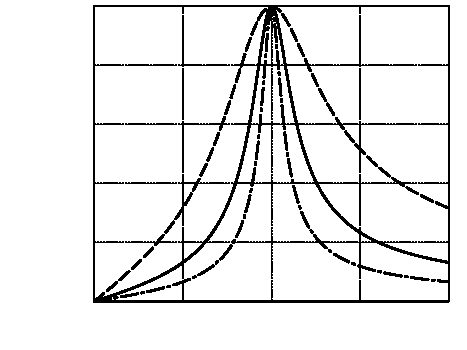
\includegraphics[width=0.25\textwidth]{9}
%	\caption{}
%	\figmark{vec-sum}
%\end{wrapfigure}

%В процессе колебаний остаётся неизменным  направление суммарного вектора $\mathbf{S}=\mathbf{S}_0+\mathbf{S}_1+\mathbf{S}_2$, изменяется лишь его длина (от максимального значения $a_0(1+m)$ до минимального значения $a_0(1-m)$), что соответствует амплитудной модуляции.
%

\todo [author=Tiffani]{Для задач неплохо было бы сделать специальную секцию (оформить в sty) с возможностью автоматической ссылки}
\important{Задача 1.} Рассмотрим теперь пример фазовой модуляции (колебание, модулированное по фазе):

\begin{equation}
	\eqmark{6.10}
	f(t)=a_0\cos(\omega_0t+\varphi(t)),\qquad \text{где}\quad \varphi(t)=m\cos\Omega t.
\end{equation}
Константа $m$~--- \important{глубина модуляции фазы}~--- определяет диапазон изменения начальной фазы (от $-m$ до $+m$) или
(если обратиться к векторной диаграмме) <<амплитуду качания>> вектора $\vec{S}$ (рис. ????).%\figref{6}б%. 
\todo [author=Tiffani]{Ссылка на несуществующий рисунок (исключен из главы по правкам Локшина)}
Используя известное тригонометрическое тождество

\begin{equation*}
	\cos(\alpha+\beta)=\cos\alpha\cos\beta-\sin\alpha\sin\beta,
\end{equation*}
запишем $f(t)$ в виде

\begin{equation*}
	f(t)=a_0\bigl(\cos\omega_0t\cos\varphi(t)-\sin\omega_0t\sin\varphi(t)\bigr).
\end{equation*}
В общем случае закон модуляции \eqref{6.10} приводит к довольно сложному спектру (с большим числом слагаемых гармонических
колебаний). Мы рассмотрим случай $m\ll 1$ (малая глубина модуляции фазы), когда можно использовать приближённые
выражения: $\cos\varphi(t)\approx 1$, $\sin\varphi(t)\approx\varphi(t)$ (мы отбрасываем величины порядка $m^2$ и выше). Тогда

\begin{equation*}
	f(t)=a_0\cos\omega_0t-a_0 m\sin\omega_0t\cos\Omega t,
\end{equation*}
или (т.~к. $2\sin\alpha\cos\beta=\sin(\alpha+\beta)+\sin(\alpha-\beta)$):
\begin{multline}
	\eqmark{6.11}
	f(t)=a_0\cos\omega_0t+\frac{ma_0}{2}\cos\left((\omega_0+\Omega)t+\frac{\pi}{2}\right)+\\
	+\frac{ma_0}{2}\cos\left((\omega_0-\Omega)t+\frac{\pi}{2}\right).
\end{multline}

Это и есть искомое представление колебания $f(t)$ в виде суммы гармонических колебаний.

Сравним формулы \eqref{6.9} и \eqref{6.11}. Первая из них~--- разложение в спектр колебания, модулированного по амплитуде,
вторая~--- колебания, модулированного по фазе. Эти колебания сильно различаются по форме (сравните осциллограммы на
рис.~\figref{modulated oscillation}б и \figref{modulated oscillation}в), однако их спектры весьма похожи.

\begin{wrapfigure}{r}{0.35\textwidth}
	\small
	\psfrag{a}[ct]{$\omega_0$}
	\psfrag{b}[ct]{$-\omega_0$}
	\psfrag{c}[ct]{$\omega_0-\Omega$}
	\psfrag{d}[ct]{$\omega_0+\Omega$}
	\psfrag{o}[ct]{0}
	\psfrag{1}{$a_0$}
	\psfrag{2}{$\frac{ma_0}{2}$}
	\psfrag{3}{$\frac{a_0}{2}$}
	\psfrag{4}{$\frac{ma_0}{4}$}
	\psfrag{x}[tl]{$\omega$}
	\psfrag{y}{$a_n$}
	\psfrag{z}{$c_n$}
	\psfrag{A}{а)}
	\psfrag{B}{б)}
	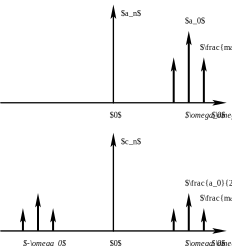
\includegraphics[width=0.25\textwidth]{Chapter_6/10}
	\caption{}
	\figmark{spectrum-modulated}
\end{wrapfigure}

В обоих случаях в правой части три слагаемых, три гармонических колебания, имеющих одинаковые частоты ($\omega_0$,
$\omega_0\pm\Omega$) и амплитуды ($a_0$~--- несущие колебания, $ma_0/2$~--- боковые гармоники). Различие выглядит
небольшим: боковые гармоники отличаются фазовым сдвигом $\frac{\pi}{2}$. Однако это различие приводит к кардинальному
отличию в форме (в осциллограмме $f(t)$) результирующего сигнала. 

%Правки. Локшин
%Векторные диаграммы на рис. \figref{vec-diagram} поясняют этот результат: поворот векторов $\mathbf{S}_1$ и $\mathbf{S}_2$ относительно вектора $\mathbf{S}_0$ на $\frac{\pi}{2}$ (рис. \figref{vec-diagram}а, ср. с рис. \figref{\vec-sum}а) приводит к тому, что с течением времени (рис. \figref{vec-diagram}б, в, г) суммарный вектор (изображён пунктиром) изменяет угол наклона, не изменяя (с точностью до величины порядка $m^2$) своей длины, что и соответствует фазовой модуляции. Этот пример подчёркивает, какую огромную роль играют фазовые соотношения при сложении колебаний.

%\begin{wrapfigure}{r}{0.35\textwidth}
%	\psfrag{A}[tc]{а)}
%	\psfrag{B}[tc]{б)}
%	\psfrag{C}[tc]{в)}
%	\psfrag{D}[tc]{г)}
%	\psfrag{0}[tb]{$\mathbf{S}_0$}
%	\psfrag{1}[lb]{$\mathbf{S}_1$}
%	\psfrag{2}[lt]{$\mathbf{S}_2$}
%	\psfrag{a}[tc]{$t=0$}
%	\psfrag{b}[tc]{$t=\frac{T}{8}$}
%	\psfrag{c}[tc]{$t=\frac{T}{4}$}
%	\psfrag{d}[tc]{$t=\frac{T}{2}$}
%	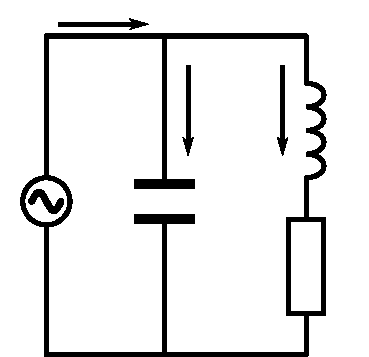
\includegraphics[width=0.25\textwidth]{11}
%	\caption{}
%	\figmark{vec-diagram}
%\end{wrapfigure}
%

Итак, изменив фазу несущего колебания (или боковых гармоник) на  $\frac{\pi}{2}$, мы можем преобразовать колебание,
модулированное по фазе, в амплитудно-модулированное колебание. Это известный в радиотехнике <<приём с изменением фазы несущей>>.

Читатель может самостоятельно проанализировать <<приём без несущей>>: что представляет собой модулированное колебание
$f(t)$, если <<убрать>> первое слагаемое~--- несущее колебание $a_0\cos\omega_0t$?

\labsection{Спектр периодического процесса}

Рассмотрим теперь периодический колебательный процесс общего вида $f(t)=f(t+T)$, где $T$~--- период процесса. В этом
случае функция $f(t)$ может быть представлена суммой гармонических колебаний с кратными частотами $\omega_n=n\omega_0$,
где $T=2\pi/\omega_0$:

\begin{equation}
	\eqmark{6.12}
	f(t)=\sum_n c_n e^{in\omega_0 t}.
\end{equation}
Действительно, для любого $t$ функция \eqref{6.12} повторяет своё значение через время $T$, поскольку

\begin{equation*}
	e^{in\omega_0(t+T)}=e^{in\omega_0t}e^{in\omega_0T}=e^{i2\pi n}e^{in\omega_0t}=e^{in\omega_0t}.
\end{equation*}
Спектр $\{c_n\}$ можно найти следующим образом: домножим обе части равенства \eqref{6.12} на $e^{-im\omega_0 t}$ и
проинтегрируем по $t$ за время, равное периоду (от $-T/2$ до $+T/2)$. Получим

\begin{equation*}
	\int_{-T/2}^{T/2} f(t)e^{-im\omega_0t}\,dt=\sum_n c_n\int_{-T/2}^{T/2} e^{i(n-m)\omega_0 t}\,dt.
\end{equation*}

Легко проверить, что интеграл в правой части равенства есть

\begin{equation*}
	\int_{-T/2}^{T/2}e^{i(n-m)\omega_0 t}dt =
	\begin{cases}
		0 & \text{при}~ n\ne m,\\
		T & \text{при}~ n = m.\\
	\end{cases}
\end{equation*}

(Интеграл от функций $\cos(n-m)\omega_0t$ и $\sin(n-m)\omega_0t$ за время $T$, равное целому числу периодов колебания этих
функций, равен 0 при $n\ne m$.) Следовательно, получаем

\begin{equation}
	\eqmark{6.13}
	c_m=\frac{1}{T}\int_{-T/2}^{T/2} f(t)e^{-im\omega_0 t}\,dt.
\end{equation}

Формула \eqref{6.13} даёт правило нахождения коэффициентов разложения периодической функции в ряд Фурье.

\important{Задача 2.} Найти спектр периодической последовательности прямоугольных импульсов длительности $\tau$ с периодом следования импульсов $T>\tau$ (рис.~\figref{meander}).

\begin{wrapfigure}[]{r}{0.4\textwidth}
	\psfrag{x}{$t$}
	\psfrag{1}[rb]{1}
	\psfrag{f}{$f(t)$}
	\psfrag{a}[cb]{$\tau$}
	\psfrag{b}[cb]{$T$}
	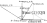
\includegraphics[width=0.35\textwidth]{Chapter_6/12}
	\caption{}
	\figmark{meander}
\end{wrapfigure}
Используя \eqref{6.13}, находим
\begin{equation*}
	c_n =\frac{1}{T}\int_{-\tau/2}^{\tau/2} e^{-in\omega_0 t}\,dt
\end{equation*}
(на интервале интегрирования $T/2\le t \le T/2$ функция $f(t)$ отлична от нуля и равна единице лишь в области
$|t|<\tau/2$). 

%Правки. Локшин
%Далее
%\begin{multline*}
%	\l c_n =\frac{1}{T}\int_{-\tau/2}^{\tau/2} \frac{e^{-in\omega_0 t}}{-in\omega_0}\,d(-in\omega_0t)=
%\left.\frac{1}{T}\frac{1}{-in\omega_0}\,e^{-in\omega_0 t}\right|^{\tau/2}_{-\tau/2}=\\
%\r=2\frac{\tau}{2T}\left[\frac{e^{in\omega_0\tau/2}-e^{-in\omega_0\tau/2}}{2in\omega_0\tau/2}\right].
%\end{multline*}
%

Окончательно находим
\begin{equation}
	\eqmark{6.14}
	c_n=\frac{\tau}{T}\left(\frac{\sin n\omega_0\tau/2}{n\omega_0\tau/2}\right).
\end{equation}

\begin{figure}[h!]
	\small
	\psfrag{x}{$\omega$}
	\psfrag{y}{$c_n$}
	\psfrag{0}[tr]{0}
	\psfrag{1}[ct]{$\vphantom{2}\omega_0$}
	\psfrag{2}[ct]{$2\omega_0$}
	\psfrag{c}{$C(\omega)$}
	\psfrag{d}[ct]{$2\Delta\omega$}
	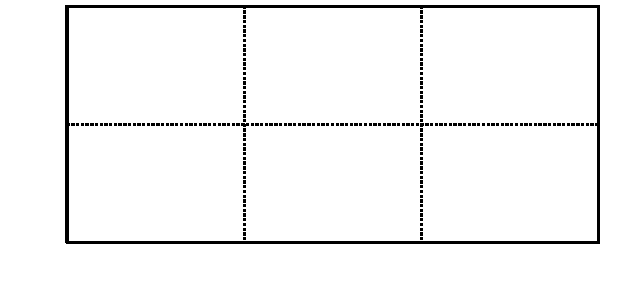
\includegraphics[width=1.0\textwidth]{Chapter_6/13}
	\caption{}
	\figmark{spectrum-meander}
\end{figure}

Спектр $\{c_n\}$ показан на рис.~\figref{spectrum-meander}. Пунктирной кривой изображена функция

\begin{equation*}
	C(\omega) =\frac{\tau}{T}\left(\frac{\sin\omega\tau/2}{\omega\tau/2}\right).
\end{equation*}

Очевидно, при $\omega=n\omega_0$ эта функция принимает значение, равное $c_n$: $c_n=C(n\omega_0)$. Полуширина $\Delta
\omega$ главного максимума этой функции определяется условием $\sin\omega\tau/2=0$:

\begin{equation*}
	\Delta\omega \cdot \frac{\tau}{2}=\pi\qquad \text{или} \qquad \Delta \omega \cdot \tau =2\pi.
\end{equation*}

Рисунок соответствует ситуации, когда $3\omega_0=\Delta\omega$, $T=3\tau$. Как видно из рисунка, спектральные гармоники,
имеющие заметную амплитуду, сосредоточены в интервале частот $|\omega|\lesssim \Delta\omega=2\pi/\tau$.

\labsection{Спектр непериодического сигнала}

Рассмотрим задачу разложения в спектр произвольного сигнала $f(t)$.

Оказывается, что произвольный сигнал не может быть представлен в виде \eqref{6.5} либо \eqref{6.6}, т.~е. в виде суммы
гармонических колебаний с дискретным набором частот $\omega_n$. В общем случае необходим непрерывный набор гармоник,
необходимо суммировать гармонические колебания, частоты которых непрерывно заполняют некоторый (быть может, бесконечный)
интервал частот. То есть необходимо иметь не только колебания с частотами $\omega_1$, $\omega_2$, $\dots$, $\omega_n$,
но также и все частоты в промежутке между ними. При этом ряд \eqref{6.5} заменяется интегралом Фурье:

\begin{equation}
	\eqmark{6.15}
	f(t)=\frac{1}{2\pi}\int_{-\infty}^\infty C(\omega)e^{i\omega t}\,d\omega.
\end{equation}

Множитель $C(\omega)=a(\omega)e^{i\varphi(\omega)}$ показывает, с каким весом (т.~е. с какой амплитудой $a(\omega)$ и с
какой начальной фазой $\varphi(\omega)$) необходимо складывать гармонические колебания разных частот, чтобы при суммировании
(интегрировании) образовать заданный сигнал $f(t)$. Функция $C(\omega)$ называется \important{спектром} (или
\important{преобразованием Фурье}) сигнала $f(t)$.

Как найти спектр, если сигнал $f(t)$ известен? Приведём формулу, вывод которой дан в п.~\r{vFur}:
\todo [author=Tiffani]{Ссылка на неизвестный пункт ``Приведём формулу, вывод которой дан в п.~\r{vFur}''}
\begin{equation}
	\eqmark{6.16}
	C(\omega)=\int_{-\infty}^\infty f(t)e^{-i\omega t}\,dt.
\end{equation}

Соотношение \eqref{6.16} математики называют \important{прямым преобразованием Фурье}, а формулу \eqref{6.15}~--- \important{обратным
преобразованием Фурье}. Связь \eqref{6.15} между функциями $f(t)$ и $C(\omega)$ символически записывается в виде
$f(t)\leftrightarrow C(\omega)$.

Как ясно из \eqref{6.16}, спектр действительной функции ($f(t)\equiv f^*(t)$) обладает определённой симметрией:
$C(\omega)=C^*(-\omega)$ и, следовательно, $|C(\omega)|=|C(-\omega)|$ ($*$~--- знак комплексного сопряжения). Математики называют это
свойство \important{эрмитовостью}.

\important{Задача 3.} Разложение в спектр прямоугольного импульса длительности $\tau$ (рис.~\figref{spectrum-one meander}а). Используя \eqref{6.16}, получаем

\begin{equation*}
	C(\omega)=\int_{-\tau/2}^{\tau/2} e^{-i\omega t}\,dt=\frac{1}{-i\omega}\int_{-\tau/2}^{\tau/2} e^{-i\omega t}\,
d(-i\omega t)=\tau\frac{\sin\omega\tau/2}{\omega\tau/2}.
\end{equation*}

Функция $C(\omega)$ показана на рис.~\figref{spectrum-one meander}б.
\todo [author=Tiffani]{Замечание. Локшин: ``Этот график (справа на рис. 6.9) должен совпадать с графиком пунктирной линии на рис. 13'' (имеется в виду рис. 13.eps спектр меандров.)}
\begin{figure}[h!]
	\psfrag{f}{$f(t)$}
	\psfrag{t}{$t$}
	\psfrag{T}[ct]{$\tau$}
	\psfrag{1}{1}
	\psfrag{F}{$C(\omega)$}
	\psfrag{w}{$\omega$}
	\psfrag{d}[cc]{$2\Delta\omega$}
	\psfrag{a}[bc]{$\frac{2\pi}{\tau}$}
	\psfrag{b}[bc]{$\llap{$-$}\frac{2\pi}{\tau}$}
	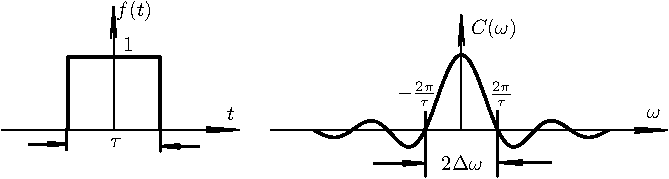
\includegraphics[width=1.0\textwidth]{Chapter_6/14}
	\caption{}
	\figmark{spectrum-one meander}
\end{figure}

Полезно сравнить спектр отдельного импульса со спектром периодической последовательности одинаковых импульсов (рис.~\figref{spectrum-meander}):
спектр импульса $C(\omega)$ (с множителем $1/T$) представляет собой <<огибающую>> частокола спектральных компонент $c_n$
периодической последовательности импульсов. Вместо дискретного спектра $\{c_n\}$ получаем непрерывный спектр $C(\omega)$.

Модуль функции $C(\omega)$ определяет амплитуды гармонических колебаний разных частот, сумма которых образует импульс
$f(t)$. Как видно из графика, основной вклад дают гармонические колебания, частоты которых заполняют интервал
$|\Delta\omega|<2\pi/\tau$. Это~--- полуширина главного максимума функции
$\frac{\sin\omega\tau/2}{\omega\tau/2}$. Диапазон частот $\Delta\omega$ можно назвать \important{шириной спектра} $C(\omega)$.

Мы получили замечательное соотношение, связывающее между собой длительность сигнала с шириной его спектра:

\begin{equation}
	\eqmark{6.17}
	\tau \cdot \Delta\omega \approx 2\pi.
\end{equation}

Это соотношение имеет универсальный характер. Оно оказывается справедливым по порядку величины для произвольного сигнала
$f(t)$. Чем больше длительность сигнала (либо больше интервал времени, в течение которого происходит его заметное
изменение), тем \'уже спектр сигнала $\Delta\omega$, и, наоборот, чем короче сигнал (или быстрее происходит изменение
сигнала), тем шире его спектр, т.~е. требуется более широкий интервал частот гармонических колебаний, образующих в сумме
данный сигнал. В этом состоит смысл замечательного соотношения \eqref{6.17}, которое называется \important{соотношением
неопределённостей}.
\begin{figure}[h!]
	\psfrag{x}{$\omega$}
	\psfrag{y}{$C_0(\omega)$}
	\psfrag{z}{$Z(\omega)$}
	\psfrag{0}[tc]{0}
	\psfrag{d}[tc]{$2\Omega$}
	\psfrag{w}[tc]{$\omega_0$}
	\psfrag{a}[cb]{$\llap{$-$}\Omega$}
	\psfrag{b}[cb]{$\Omega$}
	\psfrag{A}{а)}
	\psfrag{B}{б)}
	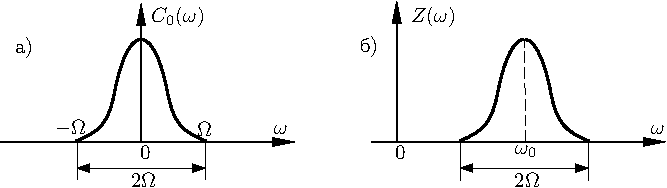
\includegraphics[width=1.0\textwidth]{Chapter_6/15}
	\caption{}
	\figmark{task-shift-spectrum}
\end{figure}

\important{Задача 4.} Спектр функции $f_0(t)$ есть $C_0(\omega)$: $f_0(t)\leftrightarrow C_0(\omega)$. Найти спектр $C(\omega)$ функции $f(t)=f_0(t)e^{i\omega_0t}$.

Согласно \eqref{6.16} запишем
\begin{equation}
	\eqmark{6.18}
	C(\omega)=\int_{-\infty}^\infty f_0(t)e^{i\omega_0 t}\cdot e^{-i\omega t}\,dt=\int_{-\infty}^\infty
f_0(t)e^{-i(\omega-\omega_0)t}\,dt=C_0(\omega-\omega_0),
\end{equation}
т.~е. спектр переносится по оси частот на величину $\omega_0$ (рис.~\figref{task-shift-spectrum}).

Из формулы \eqref{6.18} ясно, что, если спектр функции $f_0(t)$ локализован в области частот $|\omega|\le\Omega$ (рис. \figref{task-shift-spectrum}а),
то спектр функции $f(t)$ не содержит отрицательных частот (рис. \figref{task-shift-spectrum}б) $С(\omega)\equiv 0$ при $\omega<0$, если
$\omega_0>\Omega$.

%Правки. Локшин
%\textbf{Задача 6.} Спектр функции $f_0(t)$ есть $C_0(\omega)$: $f_0(t)\leftrightarrow C_0(\omega)$. Найти спектр функции $f(t)=f_0(t-\tau)$.

%Имеем
%\begin{equation*}
%	C(\omega)=\int_{-\infty}^\infty f_0(t-\tau)e^{-i\omega t}\,dt.
%\end{equation*}
%После замены переменных $t'=t-\tau$ ($dt=dt'$) получаем

%\begin{equation*}
%	C(\omega)=\int_{-\infty}^\infty f_0(t') e^{-i\omega(t'+\tau)}\,dt'.
%\end{equation*}
%Множитель $e^{-i\omega\tau}$ (не зависящий от переменной интегрирования $t'$) выносится из-под знака интеграла:

%\begin{equation}
%	\eqmark{task-freq-shift}
%	C(\omega)=e^{-i\omega\tau}\int_{-\infty}^\infty f_0(t')e^{-i\omega t'}\,dt'=C_0(\omega)\cdot e^{-i\omega\tau},
%\end{equation}
%или символически $f_0(t-\tau) \leftrightarrow C_0(\omega)e^{-i\omega\tau}$, т.е. смещение сигнала во времени на $\tau$ (запаздывание) приводит к умножению его спектра на $e^{-i\omega\tau}$ (теорема смещения).
%

\begin{figure}[h!]
	\psfrag{x}{$\omega$}
	\psfrag{y}{$C_0(\omega)$}
	\psfrag{z}{$C(\omega)$}
	\psfrag{a}[ct]{$-\omega_0$}
	\psfrag{b}[ct]{$\omega_0$}
	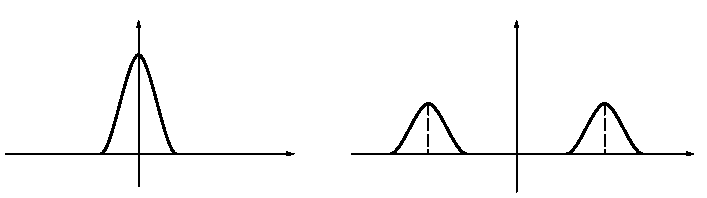
\includegraphics[width=1.0\textwidth]{Chapter_6/15b}
	\caption{}
	\figmark{task-2shift-spectrum-cos}
\end{figure}
\begin{figure}[h!]
	\psfrag{t}{$t$}
	\psfrag{f}{$f_0(t)$}
	\psfrag{F}{$f(t)$}
	\psfrag{a}[ct]{$\llap{$-$}\frac{\tau}{2}$}
	\psfrag{b}[ct]{$\frac{\tau}{2}$}
	\psfrag{A}{а)}
	\psfrag{B}{б)}
	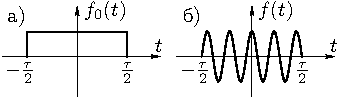
\includegraphics[width=1.0\textwidth]{Chapter_6/16}
	\caption{}
	\figmark{task-meander-train}
\end{figure}

\important{Задача 5.} Пусть $f_0(t)\leftrightarrow C_0(\omega)$. Найти спектр $C(\omega)$ функции $f(t)=f_0(t)\cos\omega_0t$.

Используя формулу Эйлера, запишем
\begin{equation*}
	f(t)=\frac{1}{2}f_0(t)e^{i\omega_0t}+\frac{1}{2}f_0(t)e^{-i\omega_0t}.
\end{equation*}

Согласно решению задачи 4, имеем
\begin{equation}
	\eqmark{6.19}
	C(\omega)=\frac{1}{2}C_0(\omega-\omega_0)+\frac{1}{2}C_0(\omega+\omega_0),
\end{equation}
т.~е. спектр $C_0(\omega)$ (умноженный на 1/2) переносится по оси частот влево и вправо на несущую частоту $\omega_0$
(рис.~\figref{task-2shift-spectrum-cos}). В частности, пусть $f_0(t)$~--- прямоугольный импульс длительности $\tau$ (рис.~\figref{task-meander-train}а):
\begin{equation*}
	f_0(t)=P_{\tau}(t)=
	\begin{cases}
		1 & \text{при}~|t|\le\tau/2,\\
		0 & \text{при}~|t|>\tau/2.\\
	\end{cases}
\end{equation*}

Тогда $f(t)=f_0(t)\cos\omega_0 t$~--- обрывок косинусоиды (цуг) длительности $\tau$ (рис.~\figref{task-meander-train}б). Согласно \eqref{6.19},
получаем
\begin{equation*}
	C(\omega)=\frac{\tau}{2}\left[\frac{\sin(\omega-\omega_0)\tau/2}{(\omega-\omega_0)\tau/2}\right]+
\frac{\tau}{2}\left[\frac{\sin(\omega+\omega_0)\tau/2}{(\omega+\omega_0)\tau/2}\right],
\end{equation*}
где $C_0(\omega)=\tau\left[\frac{\sin\omega\tau/2}{\omega\tau/2}\right]$~--- спектр импульса $f_0(t)$ (см. задачу 3).

\begin{figure}
%	\centering
	\psfrag{p}[br]{$\tau$}
	\psfrag{q}{$\tau/2$}
	\psfrag{w}{$\omega$}
	\psfrag{f}{$C_0(\omega)$}
	\psfrag{F}{$C(\omega)$}
	\psfrag{a}[ct]{$\llap{$-$}\omega_0$}
	\psfrag{b}[ct]{$\omega_0$}
	\psfrag{A}{а)}
	\psfrag{B}{б)}
	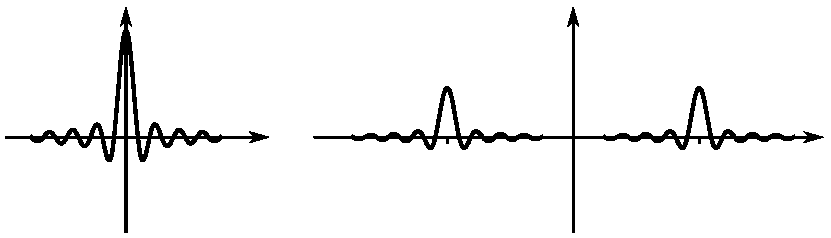
\includegraphics[width=1.0\textwidth]{Chapter_6/17}
	\caption{}
	\figmark{task-meander-train-spectrum}
\end{figure}

Спектры $C_0(\omega)$ и $C(\omega)$ представлены на рис.~\figref{task-meander-train-spectrum}.

\labsection{Линейная фильтрация (спектральный метод)}
Ещё раз опишем алгоритм решения задачи линейной фильтрации (спектральный метод).
\begin{enumerate} 
	\item Первый шаг~--- представление входного сигнала фильтра в виде суперпозиции гармонических колебаний: либо в виде ряда Фурье \eqref{6.5}, либо интеграла Фурье \eqref{6.15}. Спектр $C(\omega)$ входного сигнала $f(t)$ находится с помощью соотношений \eqref{6.13} или \eqref{6.16}.

В случае дискретного спектра, например периодической функции $f(t)$, находим набор коэффициентов $c_n$ ряда Фурье с
помощью формулы \eqref{6.14}.

	\item Второй шаг~--- нахождение частотной характеристики фильтра $H(\omega)$, т.~е. отклика фильтра на гармоническое
внешнее воздействие единичной амплитуды:
\begin{equation*}
	e^{i\omega t}\to\fbox{$L$}\to H(\omega)e^{i\omega t}.
\end{equation*}

	\item Суммируя отклики на каждое гармоническое слагаемое входного сигнала $c_n e^{i\omega_n t}$

\begin{equation*}
	c_n e^{i\omega_n t} \to\fbox{$L$}\to c_n H(\omega_n)e^{i\omega_n t},
\end{equation*}
находим результирующий выходной сигнал фильтра $g(t)$ (отклик на заданное входное воздействие $f(t)$):

\begin{equation}
	\eqmark{6.20}
	g(t)=\sum_n c_n H(\omega_n)e^{i\omega_n t}.
\end{equation}

В случае непрерывного спектра:

\begin{equation*}
	f(t)=\frac{1}{2\pi}\int_{-\infty}^\infty C(\omega)e^{i\omega t}\,d\omega,
\end{equation*}
отклик на каждое гармоническое слагаемое входного сигнала $\frac{1}{2\pi} C(\omega_n)e^{i\omega_n t}\,d\omega$ есть

\begin{equation*}
	\frac{1}{2\pi}C(\omega_n)e^{i\omega_n t}\,d\omega
\to\fbox{$L$}\to\frac{1}{2\pi}C(\omega_n)H(\omega_n)e^{i\omega_nt}\,d\omega.
\end{equation*}

Суммируя отклики, получаем

\begin{equation}
	\eqmark{6.21}
	g(t)=\frac{1}{2\pi}\int C(\omega)H(\omega)e^{i\omega t}\,d\omega.
\end{equation}

Выходной сигнал фильтра $g(t)$ (как и любой сигнал) можно представить либо в виде ряда Фурье:

\begin{equation}
	\eqmark{6.22}
	g(t)=\sum b_n e^{i\omega_n t},
\end{equation}
либо в виде интеграла Фурье:

\begin{equation}
	\eqmark{6.23}
	g(t)=\frac{1}{2\pi}\int B(\omega)e^{i\omega t}\,d\omega.
\end{equation}
Из сравнения \eqref{6.20} и \eqref{6.22}, \eqref{6.21} и \eqref{6.23} следует, что спектр выходного сигнала (набор коэффициентов
разложения $b_n$ в случае дискретного спектра) либо функция $B(\omega)$ (в случае непрерывного спектра) находятся с
помощью равенств

\begin{equation}
	\eqmark{6.24}
	b_n=c_n H(\omega_n),\qquad B(\omega)=C(\omega)\cdot H(\omega),
\end{equation}
которые лежат в основе спектрального метода решения задачи линейной фильтрации.
\end{enumerate}

%Правки. Локшин
%В частности, равенства \eqref{output signal-spectrum} подсказывают путь решения \important{задачи селекции}, которая возникает при приёме радиосигналов. Пусть на вход колебательного контура приёмника поступают сигналы двух радиостанций, ведущих передачи на несущих частотах $\omega_0$ и $\omega_1$. Это~--- модулированные колебания

%\begin{equation*}
%	f_s(t)=a(t)\cos(\omega_0t+\varphi_1(t))
%\end{equation*}
%и
%\begin{equation*}
%	f_n(t)=a(t)\cos(\omega_1t+\varphi_2(t)).
%\end{equation*}
%Их спектры $C_s(\omega)$ и $C_n(\omega)$. Требуется выделить полезный сигнал $f_s(t)$ и отсеять помехи (сигнал $f_n(t)$).

%Требования, предъявляемые к частотной характеристике контура, вытекают из соотношений \eqref{output signal-spectrum}. Во-первых, контур необходимо настроить на несущую частоту сигнала $f_s(t)$, т.~е. резонансная частота контура $\omega_р$ должна совпадать с $\omega_0$: $\omega_р\simeq\omega_0$. При этом добротность контура $Q$ должна быть достаточно большой, чтобы в пределы полосы пропускания контура $\Delta\omega=\frac{\omega_0}{Q}$ не попали спектральные компоненты помех $\omega_1$, $|\omega_1-\omega_0|>\Delta\omega_к$. С другой стороны, чтобы полезный сигнал был принят без искажений, необходимо, чтобы полоса частот полезного сигнала $\Delta\Omega$, определяемая характерным временем $\tau$ изменения функций $a(t)$ и $\varphi(t)$, описывающих закон модуляции ($\Delta\Omega\cdot\tau\approx 2\pi$~--- соотношение неопределённостей), была меньше полосы пропускания контура $\Delta\Omega\ll\Delta\omega_к$. Всем этим условиям удовлетворяет частотная характеристика, изображённая на рис. \figref{freq characteristic} (показаны сигналы $f_s(t)$ и $f_n(\omega)$ с дискретными спектрами $C_s(\omega)$ и $C_n(\omega)$).

%\begin{wrapfigure}{r}{1.0\textwidth}
%	\psfrag{x}{$\omega$}
%	\psfrag{d}[ct]{$\omega_0$}
%	\psfrag{e}[ct]{$\omega_1$}
%	\psfrag{f}[cb]{$\Delta\omega_к$}
%	\psfrag{g}[cb]{$\Delta\Omega$}
%	\psfrag{y}[cr]{$Q$}
%	\psfrag{1}[cr]{1}
%	\psfrag{a}[cl]{$H(\omega)$}
%	\psfrag{b}[cl]{$C_s(\omega)$}
%	\psfrag{c}[cl]{$C_n(\omega)$}
%	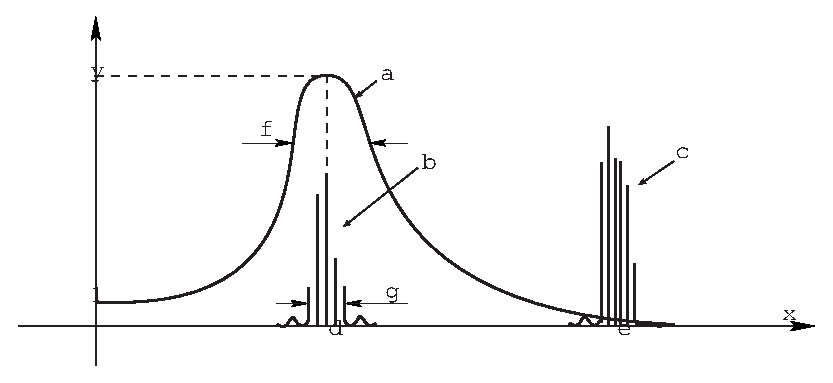
\includegraphics[width=1.0\textwidth]{21}
%	\caption{}
%	\figmark{freq characteristic}
%\end{wrapfigure}

%Спектр выходного сигнала находим с помощью \eqref{output signal-spectrum}:

%\begin{equation*}
%	B(\omega)=\left[F_s(\omega)+F_n(\omega)\right]\cdot H(\omega)\simeq F_s(\omega)\cdot H(\omega_р)\simeq Q\cdot C_s(\omega).
%\end{equation*}
%Спектральные компоненты на частотах $\omega\approx\omega_1$ оказываются подавленными, поскольку $B(\omega)=C_n(\omega)\cdot H(\omega)\simeq 0$. Действительно, из выражения для частотной характеристики резонансного контура (см. задачу 1) следует (при $Q\gg 1$): $H(\omega)\approx 1$ при $\omega\ll\omega_р$, $H(\omega)\approx Q$ при $\omega\approx\omega_р=\omega_0$ и $H(\omega)\approx (\omega_к/\omega)^2$ при $\omega\gg\omega_р$. Поэтому первое слагаемое

%\begin{equation*}
%	C_s(\omega)H(\omega)\simeq C_s(\omega)Q,
%\end{equation*}
%а второе

%\begin{equation*}
%	C_n(\omega)H(\omega)\simeq C_n(\omega)\left(\frac{\omega_0}{\omega}\right)^2
%\end{equation*}
%при $\omega\gg\omega_0$ пренебрежимо мало.

\begin{lab:literature}
	\item~\emph{Сивухин~Д.В.} Общий курс физики.~Т.III. Электричество --- М.:~Наука, 1983. \S~128.	
	\item~\emph{Кингсеп~А.С., Локшин~Г.Р., Ольхов~О.А.} Основы физики.~Т.I.--- М.:~Физматлит, 2007. Гл I, \S\S~1.5, 1.6, стр.~395--414
	\item~\emph{Локшин~Г.Р., Козел~С.М.} Модулированные колебания. Спектральный анализ. Линейная фильтрация --- М.:~МФТИ, 2009
\end{lab:literature}